\begin{enumerate}[label=\thesection.\arabic*.,ref=\thesection.\theenumi]
\numberwithin{equation}{enumi}
\item
Sketch the Polar Plot of
\begin{align}
G\brak{s} = \frac{1}{s\brak{1+s^{2}}}
\end{align}
\\
\solution  
Given the Open Loop Transfer Function
\begin{align}
G\brak{s} = \frac{1}{s\brak{1+s^{2}}}
\end{align}
Now we have substitute s=$\j\omega$
\begin{align}
G\brak{\j\omega} =   \frac{1}{\j\omega\brak{1-{\omega}^{2}}}
\end{align}

\item
Find the Magnitude of the Transfer Function
\begin{align}
G\brak{\j\omega} =   \frac{1}{\j\omega\brak{1-{\omega}^{2}}}
\end{align}
\begin{align}
      |G\brak{\j\omega}| = \frac{1}{|\omega\brak{1-{\omega}^{2}}|}
\end{align}
\item
Find the Phase of Transfer Function

\begin{align}
    \angle G\brak{\j\omega} = \angle G\brak{\j\omega}_{num} - \angle G\brak{\j\omega}_{den}
\end{align}
for $\omega\brak{1-{\omega}^{2}}$ $<$ 0
\begin{align}
    \angle G\brak{\j\omega} = \frac{\pi}{2}
\end{align}
for $\omega\brak{1-{\omega}^{2}}$ $>$ 0
\begin{align}
    \angle G\brak{\j\omega}) = -\frac{\pi}{2}
\end{align}
\item
Draw Polar Plot using phase of transfer function
For $\omega$=0 
\begin{align}
    \abs{G\brak{\j\omega}} = \infty
    \end{align}
\begin{align}
    \angle G\brak{\j\omega} = \frac{\pi}{2}
\end{align}
For w= $\infty$
\begin{align}
    \abs{G\brak{\j\omega}} = 0
    \end{align}
\begin{align}
    \angle G\brak{\j\omega} = \frac{\pi}{2}
\end{align}
Polar Plot drawn by varying $\omega$ from 0 to $\infty$.
\begin{figure}[!h]
  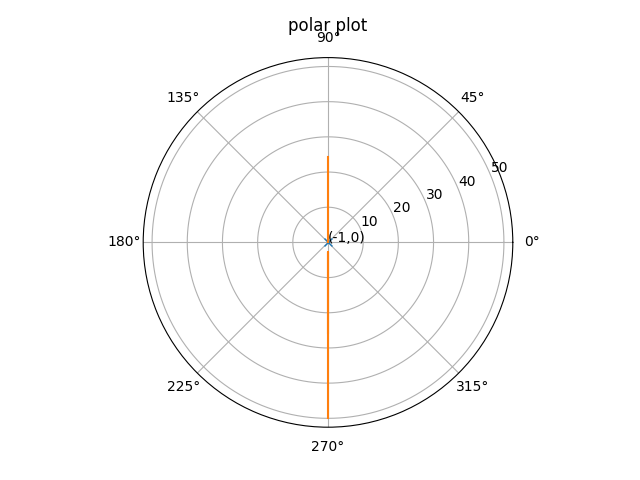
\includegraphics[width=\columnwidth]{ee18btech11023_1c.png}
  \caption{}
  \label{ee18btech11023}
\end{figure}

\item
Verify the Polar Plot the running the following Code
\begin{lstlisting}
https://github.com/srikanth2001/EE2227/tree/master/codes
\end{lstlisting}

\item
 Stability

\break for the given transfer function 
\begin{align}
    G\brak{s} = \frac{1}{s\brak{1+s^{2}}}
\end{align}
The polar plots use open loop transfer function, hence the reference point for determining
stability is shifted to (–1, 0)
\center
 If (–1,0) is exactly on the polar plot then the system is marginally stable
polar plot useful to find the stability of given transfer function
from the graph we can see that (-1,0) is lying exactly on polar plot

&
&
\center so the system is marginally stable
\end{enumerate}
